%% LaTeX-Beamer template for KIT design
%% by Erik Burger, Christian Hammer
%% title picture by Klaus Krogmann
%%
%% version 2.0
%%
%% mostly compatible to KIT corporate design v2.0
%% http://intranet.kit.edu/gestaltungsrichtlinien.php
%%
%% Problems, bugs and comments to
%% burger@kit.edu

\documentclass[18pt]{beamer}
\usetheme{kit}

%% TITLE PICTURE

% if a custom picture is to be used on the title page, copy it into the 'logos'
% directory, in the line below, replace 'mypicture' with the 
% filename (without extension) and uncomment the following line
% (picture proportions: 63 : 20, *.eps format if you use latex+dvips+ps2pdf,
% *.jpg/*.png/*.pdf if you use pdflatex)

%\titleimage{mypicture}

%% TITLE LOGO

% for a custom logo on the front page, copy your file into the 'logos'
% directory, insert the filename in the line below and uncomment it

%\titlelogo{mylogo}

% (*.eps format if you use latex+dvips+ps2pdf,
% *.jpg/*.png/*.pdf if you use pdflatex)

%% BIBTEX ICON/KEY

% if you want to see BibTeX keys in the references view instead of the symbol,
% uncomment the following line
% \usebibitemtemplate{\insertbiblabel}

% the presentation starts here

\title[Short title]{Tutorium 01: Projektplanung }
\subtitle{Softwaretechnik im SS 2011, Gruppe 2}
\author{Jürgen Walter}

\institute{Chair for Software Design and Quality}

\begin{document}

% change the following line to "ngerman" for German style date and logos
% change the following line to "english" for English style date and logos
\selectlanguage{ngerman}

%title page
\begin{frame}
\titlepage
\end{frame}

%table of contents
\frame{
\frametitle{Was machen wir heute?}
\tableofcontents
}



\section{Organisatorisches}

\subsection{Vorstellung}
\frame{
\frametitle{Wer bin ich?}
\begin{itemize}
\item Jürgen Walter
\pause
\item 8tes Semester Informatik
\pause
\item juergen.walter.halle@gmail.com
\item uxccx@student.kit.edu
\pause
\item Partnerturoren Christian Juelg und Daniel Deckers
\item \dots
\end{itemize}
}

\subsection{Übungsschein}
\frame{
\frametitle{Übungsschein}
\begin{block}{Der Übungschein ist \dots}
\begin{itemize}
\pause
\item Vorraussetzung zur Klausur
\pause
\item 6 Übungsblätter
\pause
\item 150 Punkte insgesammt 
\pause
\item mit 50 Prozent aus Übungsblättern und Programmmieraufgaben bestanden 
\end{itemize}
\end{block}
}



\section{Versionsverwaltungen}

\frame{
\frametitle{Subversion}
\begin{itemize}
\pause
\item von der Vorlesung unterstützte Versionsverwaltung
\end{itemize}
}

\frame{
\frametitle{Git}
\begin{itemize}
\pause
\item Werkzeug des Tutors ;-)
\end{itemize}
}



\section{Lastenheft}

\subsection{Gliederungsschema}

\frame{
\frametitle{Gliederungsschema}
\begin{itemize}
\item enthält die Hauptanforderungen an das Produkt (user requirements)
\item formuliert mit natürlicher Sprache, evtl. Diagramme
\item dient der Kommunikation mit dem Kunden und der Projektplanung
\end{itemize}
}

\frame{
\frametitle{Gliederungsschema}
\begin{block}{Gliederungsschema Lastenheft}
\begin{itemize}
\item1.Zielbestimmung
\item2.Produkteinsatz
\item3.Produktfunktionen
\item4.Produktdaten
\item5.Produktleistungen
\item6.Qualitätsanforderungen
\item7.Ergänzungen (weitere nichtfunktionale Eigenschaften).
\item8.Glossar (Begriffslexikon zur Beschreibung des Produktes)
\end{itemize}
\end{block}
}



\section{Ende}

\frame{
\frametitle{Nächstes Übungsblatt}
}


\frame{
\frametitle{Ende}
\begin{center}
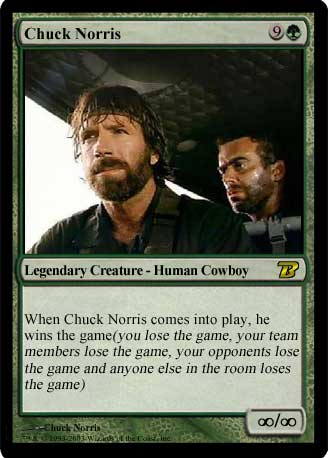
\includegraphics[width=0.4\textwidth]{pics/chuckNorris}
\end{center}

}


\end{document}
